\chapter{Árvores geradoras}

\index{árvore geradora}

Uma \key{árvore geradora} de um grafo é composta
por todos os nós do grafo e por algumas de suas 
arestas, de forma que haja um caminho 
entre quaisquer dois nós. 
Assim como as árvores em geral, as árvores geradoras são 
conectadas e acíclicas. 
Normalmente, existem várias maneiras de construir uma árvore geradora.

Por exemplo, considere o seguinte grafo:
\begin{center}
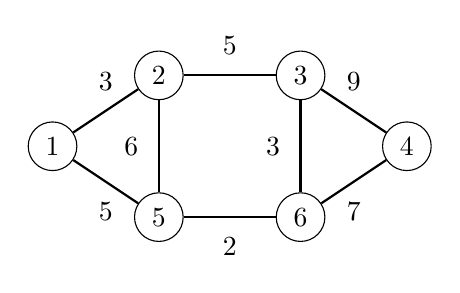
\begin{tikzpicture}[scale=0.9]
\node[draw, circle] (1) at (1.5,2) {$1$};
\node[draw, circle] (2) at (3,3) {$2$};
\node[draw, circle] (3) at (5,3) {$3$};
\node[draw, circle] (4) at (6.5,2) {$4$};
\node[draw, circle] (5) at (3,1) {$5$};
\node[draw, circle] (6) at (5,1) {$6$};
\path[draw,thick,-] (1) -- node[font=\small,label=above:3] {} (2);
\path[draw,thick,-] (2) -- node[font=\small,label=above:5] {} (3);
\path[draw,thick,-] (3) -- node[font=\small,label=above:9] {} (4);
\path[draw,thick,-] (1) -- node[font=\small,label=below:5] {} (5);
\path[draw,thick,-] (5) -- node[font=\small,label=below:2] {} (6);
\path[draw,thick,-] (6) -- node[font=\small,label=below:7] {} (4);
\path[draw,thick,-] (2) -- node[font=\small,label=left:6] {} (5);
\path[draw,thick,-] (3) -- node[font=\small,label=left:3] {} (6);
\end{tikzpicture}
\end{center}
Uma árvore geradora para o grafo é a seguinte:
\begin{center}
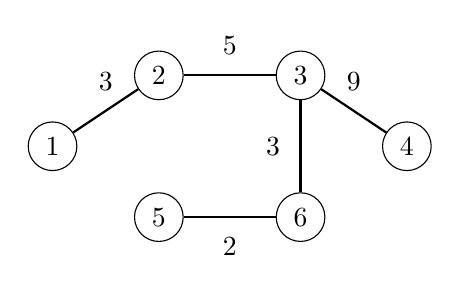
\begin{tikzpicture}[scale=0.9]
\node[draw, circle] (1) at (1.5,2) {$1$};
\node[draw, circle] (2) at (3,3) {$2$};
\node[draw, circle] (3) at (5,3) {$3$};
\node[draw, circle] (4) at (6.5,2) {$4$};
\node[draw, circle] (5) at (3,1) {$5$};
\node[draw, circle] (6) at (5,1) {$6$};
\path[draw,thick,-] (1) -- node[font=\small,label=above:3] {} (2);
\path[draw,thick,-] (2) -- node[font=\small,label=above:5] {} (3);
\path[draw,thick,-] (3) -- node[font=\small,label=above:9] {} (4);
\path[draw,thick,-] (5) -- node[font=\small,label=below:2] {} (6);
\path[draw,thick,-] (3) -- node[font=\small,label=left:3] {} (6);
\end{tikzpicture}
\end{center}

O peso de uma árvore geradora é a soma dos pesos de suas arestas.
Por exemplo, o peso da árvore geradora acima é
$3+5+9+3+2=22$.

\index{Árvore geradora mínima}

Uma \key{Árvore geradora mínima}
é uma árvore geradora cujo peso é o menor possível.
O peso de uma árvore geradora mínima para o grafo de exemplo
é 20, e tal árvore pode ser construída da seguinte forma:

\begin{center}
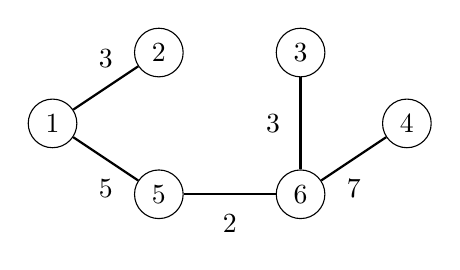
\begin{tikzpicture}[scale=0.9]
\node[draw, circle] (1) at (1.5,2) {$1$};
\node[draw, circle] (2) at (3,3) {$2$};
\node[draw, circle] (3) at (5,3) {$3$};
\node[draw, circle] (4) at (6.5,2) {$4$};
\node[draw, circle] (5) at (3,1) {$5$};
\node[draw, circle] (6) at (5,1) {$6$};

\path[draw,thick,-] (1) -- node[font=\small,label=above:3] {} (2);
\path[draw,thick,-] (1) -- node[font=\small,label=below:5] {} (5);
\path[draw,thick,-] (5) -- node[font=\small,label=below:2] {} (6);
\path[draw,thick,-] (6) -- node[font=\small,label=below:7] {} (4);
\path[draw,thick,-] (3) -- node[font=\small,label=left:3] {} (6);
\end{tikzpicture}
\end{center}

\index{Árvore geradora máxima}

De maneira semelhante, uma \key{Árvore geradora máxima}
é uma árvore geradora cujo peso é o maior possível.
O peso de uma árvore geradora máxima para o
grafo de exemplo é 32:

\begin{center}
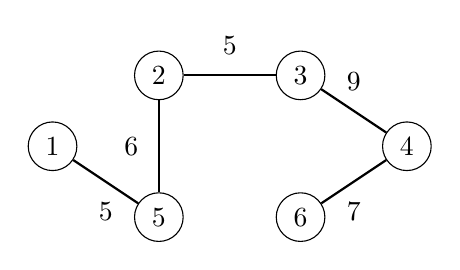
\begin{tikzpicture}[scale=0.9]
\node[draw, circle] (1) at (1.5,2) {$1$};
\node[draw, circle] (2) at (3,3) {$2$};
\node[draw, circle] (3) at (5,3) {$3$};
\node[draw, circle] (4) at (6.5,2) {$4$};
\node[draw, circle] (5) at (3,1) {$5$};
\node[draw, circle] (6) at (5,1) {$6$};
\path[draw,thick,-] (2) -- node[font=\small,label=above:5] {} (3);
\path[draw,thick,-] (3) -- node[font=\small,label=above:9] {} (4);
\path[draw,thick,-] (1) -- node[font=\small,label=below:5] {} (5);
\path[draw,thick,-] (6) -- node[font=\small,label=below:7] {} (4);
\path[draw,thick,-] (2) -- node[font=\small,label=left:6] {} (5);
\end{tikzpicture}
\end{center}

Note que um grafo pode ter várias
árvores geradoras mínimas e máximas,
então as árvores não são únicas.

Acontece que vários métodos gulosos
podem ser usados para construir árvores geradoras
mínimas e máximas.
Neste capítulo, discutimos dois algoritmos
que processam
as arestas do grafo ordenadas pelos seus pesos.
Nosso foco é encontrar árvores geradoras mínimas,
mas os mesmos algoritmos podem encontrar
árvores geradoras máximas processando as arestas em ordem inversa.

\section{Algoritmo de Kruskal}

\index{Algoritmo de Kruskal}

No \key{Algoritmo de Kruskal}\footnote{O algoritmo foi publicado em 1956
por J. B. Kruskal \cite{kru56}.}, a árvore geradora inicial
contém apenas os nós do grafo
e não contém nenhuma aresta.
Em seguida, o algoritmo percorre as arestas
ordenadas pelos seus pesos, e sempre adiciona uma aresta
à árvore se ela não criar um ciclo.

O algoritmo mantém os componentes
da árvore.
Inicialmente, cada nó do grafo
pertence a um componente separado.
Sempre que uma aresta é adicionada à árvore,
dois componentes são unidos.
Finalmente, todos os nós pertencem ao mesmo componente,
 e uma árvore geradora mínima foi encontrada.

\subsubsection{Exemplo}

\begin{samepage}
Vamos considerar como o algoritmo de Kruskal processa o
seguinte grafo:
\begin{center}
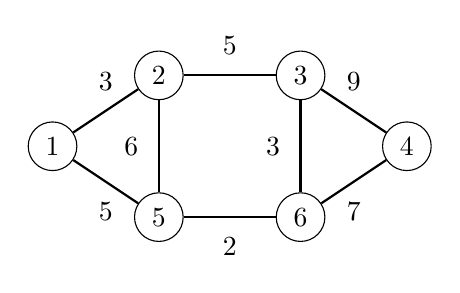
\begin{tikzpicture}[scale=0.9]
\node[draw, circle] (1) at (1.5,2) {$1$};
\node[draw, circle] (2) at (3,3) {$2$};
\node[draw, circle] (3) at (5,3) {$3$};
\node[draw, circle] (4) at (6.5,2) {$4$};
\node[draw, circle] (5) at (3,1) {$5$};
\node[draw, circle] (6) at (5,1) {$6$};
\path[draw,thick,-] (1) -- node[font=\small,label=above:3] {} (2);
\path[draw,thick,-] (2) -- node[font=\small,label=above:5] {} (3);
\path[draw,thick,-] (3) -- node[font=\small,label=above:9] {} (4);
\path[draw,thick,-] (1) -- node[font=\small,label=below:5] {} (5);
\path[draw,thick,-] (5) -- node[font=\small,label=below:2] {} (6);
\path[draw,thick,-] (6) -- node[font=\small,label=below:7] {} (4);
\path[draw,thick,-] (2) -- node[font=\small,label=left:6] {} (5);
\path[draw,thick,-] (3) -- node[font=\small,label=left:3] {} (6);
\end{tikzpicture}
\end{center}
\end{samepage}

\begin{samepage}
O primeiro passo do algoritmo é ordenar as
arestas em ordem crescente de seus pesos.
O resultado é a seguinte lista:

\begin{tabular}{ll}
\\
aresta & peso \\
\hline
5--6 & 2 \\
1--2 & 3 \\
3--6 & 3 \\
1--5 & 5 \\
2--3 & 5 \\
2--5 & 6 \\
4--6 & 7 \\
3--4 & 9 \\
\\
\end{tabular}
\end{samepage}

Depois disso, o algoritmo percorre a lista
e adiciona cada aresta à árvore se ela unir
dois componentes separados.

Inicialmente, cada nó está em seu próprio componente:

\begin{center}
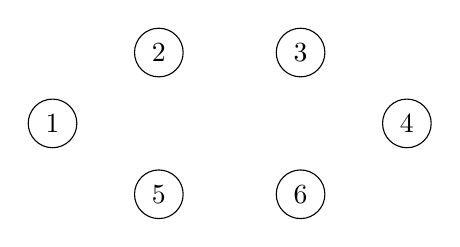
\begin{tikzpicture}[scale=0.9]
\node[draw, circle] (1) at (1.5,2) {$1$};
\node[draw, circle] (2) at (3,3) {$2$};
\node[draw, circle] (3) at (5,3) {$3$};
\node[draw, circle] (4) at (6.5,2) {$4$};
\node[draw, circle] (5) at (3,1) {$5$};
\node[draw, circle] (6) at (5,1) {$6$};
%\path[draw,thick,-] (1) -- node[font=\small,label=above:3] {} (2);
%\path[draw,thick,-] (2) -- node[font=\small,label=above:5] {} (3);
%\path[draw,thick,-] (3) -- node[font=\small,label=above:9] {} (4);
%\path[draw,thick,-] (1) -- node[font=\small,label=below:5] {} (5);
%\path[draw,thick,-] (5) -- node[font=\small,label=below:2] {} (6);
%\path[draw,thick,-] (6) -- node[font=\small,label=below:7] {} (4);
%\path[draw,thick,-] (2) -- node[font=\small,label=left:6] {} (5);
%\path[draw,thick,-] (3) -- node[font=\small,label=left:3] {} (6);
\end{tikzpicture}
\end{center}
A primeira aresta a ser adicionada à árvore é
a aresta 5--6 que cria um componente $\{5,6\}$
ao unir os componentes $\{5\}$ e $\{6\}$:

\begin{center}
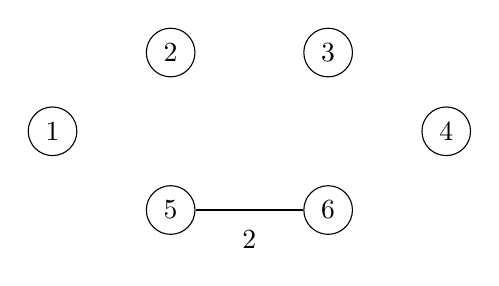
\begin{tikzpicture}
\node[draw, circle] (1) at (1.5,2) {$1$};
\node[draw, circle] (2) at (3,3) {$2$};
\node[draw, circle] (3) at (5,3) {$3$};
\node[draw, circle] (4) at (6.5,2) {$4$};
\node[draw, circle] (5) at (3,1) {$5$};
\node[draw, circle] (6) at (5,1) {$6$};

%\path[draw,thick,-] (1) -- node[font=\small,label=above:3] {} (2);
%\path[draw,thick,-] (2) -- node[font=\small,label=above:5] {} (3);
%\path[draw,thick,-] (3) -- node[font=\small,label=above:9] {} (4);
%\path[draw,thick,-] (1) -- node[font=\small,label=below:5] {} (5);
\path[draw,thick,-] (5) -- node[font=\small,label=below:2] {} (6);
%\path[draw,thick,-] (6) -- node[font=\small,label=below:7] {} (4);
%\path[draw,thick,-] (2) -- node[font=\small,label=left:6] {} (5);
%\path[draw,thick,-] (3) -- node[font=\small,label=left:3] {} (6);
\end{tikzpicture}
\end{center}
Após isso, as arestas 1--2, 3--6 e 1--5 são adicionadas de maneira similar:

\begin{center}
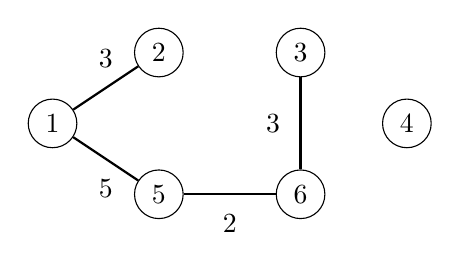
\begin{tikzpicture}[scale=0.9]
\node[draw, circle] (1) at (1.5,2) {$1$};
\node[draw, circle] (2) at (3,3) {$2$};
\node[draw, circle] (3) at (5,3) {$3$};
\node[draw, circle] (4) at (6.5,2) {$4$};
\node[draw, circle] (5) at (3,1) {$5$};
\node[draw, circle] (6) at (5,1) {$6$};

\path[draw,thick,-] (1) -- node[font=\small,label=above:3] {} (2);
%\path[draw,thick,-] (2) -- node[font=\small,label=above:5] {} (3);
%\path[draw,thick,-] (3) -- node[font=\small,label=above:9] {} (4);
\path[draw,thick,-] (1) -- node[font=\small,label=below:5] {} (5);
\path[draw,thick,-] (5) -- node[font=\small,label=below:2] {} (6);
%\path[draw,thick,-] (6) -- node[font=\small,label=below:7] {} (4);
%\path[draw,thick,-] (2) -- node[font=\small,label=left:6] {} (5);
\path[draw,thick,-] (3) -- node[font=\small,label=left:3] {} (6);
\end{tikzpicture}
\end{center}

Após esses passos, a maioria dos componentes foi unida
e há dois componentes na árvore:
$\{1,2,3,5,6\}$ e $\{4\}$.

A próxima aresta na lista é a aresta 2--3,
mas ela não será incluída na árvore, pois
os nós 2 e 3 já estão no mesmo componente.
Pelo mesmo motivo, a aresta 2--5 também não será incluída na árvore.

\begin{samepage}
Finalmente, a aresta 4--6 será incluída na árvore:

\begin{center}
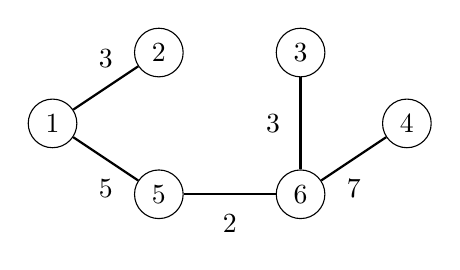
\begin{tikzpicture}[scale=0.9]
\node[draw, circle] (1) at (1.5,2) {$1$};
\node[draw, circle] (2) at (3,3) {$2$};
\node[draw, circle] (3) at (5,3) {$3$};
\node[draw, circle] (4) at (6.5,2) {$4$};
\node[draw, circle] (5) at (3,1) {$5$};
\node[draw, circle] (6) at (5,1) {$6$};

\path[draw,thick,-] (1) -- node[font=\small,label=above:3] {} (2);
%\path[draw,thick,-] (2) -- node[font=\small,label=above:5] {} (3);
%\path[draw,thick,-] (3) -- node[font=\small,label=above:9] {} (4);
\path[draw,thick,-] (1) -- node[font=\small,label=below:5] {} (5);
\path[draw,thick,-] (5) -- node[font=\small,label=below:2] {} (6);
\path[draw,thick,-] (6) -- node[font=\small,label=below:7] {} (4);
%\path[draw,thick,-] (2) -- node[font=\small,label=left:6] {} (5);
\path[draw,thick,-] (3) -- node[font=\small,label=left:3] {} (6);
\end{tikzpicture}
\end{center}
\end{samepage}

Após isso, o algoritmo não adicionará 
mais arestas, porque o grafo está conectado
e há um caminho entre quaisquer dois nós.
O grafo resultante é uma árvore geradora mínima
com peso $2+3+3+5+7=20$.

\subsubsection{Por que isso funciona?}

É uma boa pergunta por que o algoritmo de Kruskal funciona.
Por que a estratégia gulosa garante que 
encontraremos uma árvore geradora mínima?

Vamos ver o que acontece se a aresta de menor peso do
grafo \emph{não} estiver incluída na árvore geradora.
Por exemplo, suponha que uma árvore geradora
para o grafo anterior não contivesse a
aresta de menor peso 5--6.
Não sabemos a estrutura exata de tal árvore geradora,
mas em qualquer caso ela tem que conter algumas arestas.
Assuma que a árvore seria como a seguinte:

\begin{center}
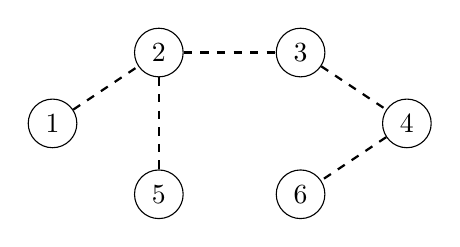
\begin{tikzpicture}[scale=0.9]
\node[draw, circle] (1) at (1.5,2) {$1$};
\node[draw, circle] (2) at (3,3) {$2$};
\node[draw, circle] (3) at (5,3) {$3$};
\node[draw, circle] (4) at (6.5,2) {$4$};
\node[draw, circle] (5) at (3,1) {$5$};
\node[draw, circle] (6) at (5,1) {$6$};

\path[draw,thick,-,dashed] (1) -- (2);
\path[draw,thick,-,dashed] (2) -- (5);
\path[draw,thick,-,dashed] (2) -- (3);
\path[draw,thick,-,dashed] (3) -- (4);
\path[draw,thick,-,dashed] (4) -- (6);
\end{tikzpicture}
\end{center}

Entretanto, não é possível que a árvore acima
seja uma árvore geradora mínima para o grafo.
O motivo disso é que podemos remover uma aresta
da árvore e substituí-la pela aresta de peso mínimo 5--6.
Isso produz uma árvore geradora cujo peso é
\emph{menor}:

\begin{center}
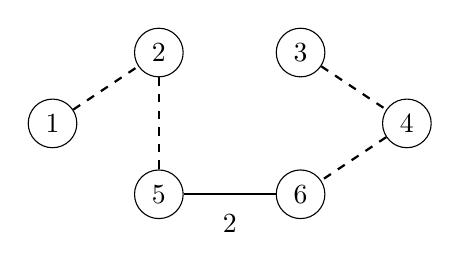
\begin{tikzpicture}[scale=0.9]
\node[draw, circle] (1) at (1.5,2) {$1$};
\node[draw, circle] (2) at (3,3) {$2$};
\node[draw, circle] (3) at (5,3) {$3$};
\node[draw, circle] (4) at (6.5,2) {$4$};
\node[draw, circle] (5) at (3,1) {$5$};
\node[draw, circle] (6) at (5,1) {$6$};

\path[draw,thick,-,dashed] (1) -- (2);
\path[draw,thick,-,dashed] (2) -- (5);
\path[draw,thick,-,dashed] (3) -- (4);
\path[draw,thick,-,dashed] (4) -- (6);
\path[draw,thick,-] (5) -- node[font=\small,label=below:2] {} (6);
\end{tikzpicture}
\end{center}

Por essa razão, é sempre ideal 
incluir a aresta de menor peso 
na árvore para produzir uma árvore geradora mínima.
Usando um argumento semelhante, podemos mostrar que também 
é ideal adicionar a próxima aresta em ordem de peso 
à árvore, e assim por diante.
Portanto, o algoritmo de Kruskal funciona corretamente e 
sempre produz uma árvore geradora mínima.

\subsubsection{Implementação}

Ao implementar o algoritmo de Kruskal, 
é conveniente usar 
a representação de lista de arestas do grafo. 
A primeira fase do algoritmo ordena as 
arestas na lista em tempo $O(m \log m)$. 
Após isso, a segunda fase do algoritmo 
constrói a árvore geradora mínima da seguinte forma:

\begin{lstlisting}
for (...) {
  if (!same(a,b)) unite(a,b);
}
\end{lstlisting}

O laço percorre as arestas na lista 
e sempre processa uma aresta $a$--$b$
onde $a$ e $b$ são dois nós. 
Duas funções são necessárias: 
a função \texttt{same} determina 
se $a$ e $b$ estão no mesmo componente, 
e a função \texttt{unite} 
une os componentes que contêm $a$ e $b$.

O problema é como implementar eficientemente 
as funções \texttt{same} e \texttt{unite}. 
Uma possibilidade é implementar a função 
\texttt{same} como uma travessia de grafo e verificar se 
podemos ir do nó $a$ ao nó $b$. 
No entanto, a complexidade de tempo de tal função 
seria $O(n+m)$
 e o algoritmo resultante seria lento, 
pois a função \texttt{same} será chamada para cada aresta no grafo.

Resolveremos o problema usando uma estrutura union-find 
que implementa ambas as funções em tempo $O(\log n)$. 
Assim, a complexidade de tempo do algoritmo de Kruskal 
será $O(m \log n)$ após ordenar a lista de arestas.

\section{Estrutura Union-Find}

\index{Estrutura union-find}

Uma \key{Estrutura union-find} mantém 
uma coleção de conjuntos. 
Os conjuntos são disjuntos, então nenhum elemento 
pertence a mais de um conjunto. 
Duas operações de tempo $O(\log n)$ são suportadas: 
a operação \texttt{unite} une dois conjuntos 
e a operação \texttt{find} encontra o representante do conjunto 
que contém um determinado elemento\footnote{A estrutura apresentada aqui 
foi introduzida em 1971 por J. D. Hopcroft e J. D. Ullman \cite{hop71}. 
Posteriormente, em 1975, R. E. Tarjan estudou uma variante mais sofisticada 
da estrutura \cite{tar75} que é discutida em muitos livros de algoritmos 
hoje em dia.}.

\subsubsection{Estrutura}

Em uma estrutura union-find, um elemento em cada conjunto 
é o representante do conjunto, 
e há uma cadeia de qualquer outro elemento do 
conjunto para o representante. 
Por exemplo, suponha que os conjuntos sejam 
$\{1,4,7\}$, $\{5\}$ e $\{2,3,6,8\}$:
\begin{center}
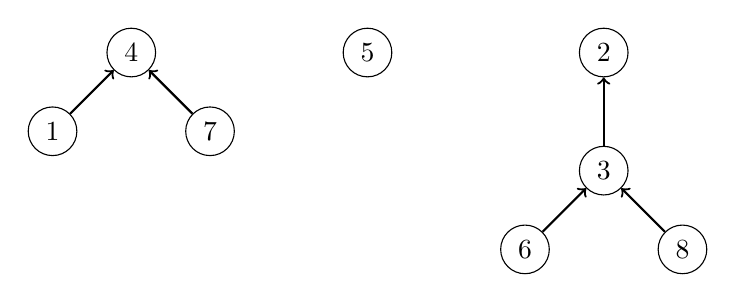
\begin{tikzpicture}
\node[draw, circle] (1) at (0,-1) {$1$};
\node[draw, circle] (2) at (7,0) {$2$};
\node[draw, circle] (3) at (7,-1.5) {$3$};
\node[draw, circle] (4) at (1,0) {$4$};
\node[draw, circle] (5) at (4,0) {$5$};
\node[draw, circle] (6) at (6,-2.5) {$6$};
\node[draw, circle] (7) at (2,-1) {$7$};
\node[draw, circle] (8) at (8,-2.5) {$8$};

\path[draw,thick,->] (1) -- (4);
\path[draw,thick,->] (7) -- (4);

\path[draw,thick,->] (3) -- (2);
\path[draw,thick,->] (6) -- (3);
\path[draw,thick,->] (8) -- (3);

\end{tikzpicture}
\end{center}
Neste caso, os representantes 
dos conjuntos são 4, 5 e 2. 
Podemos encontrar o representante de qualquer elemento 
seguindo a cadeia que começa no elemento. 
Por exemplo, o elemento 2 é o representante 
do elemento 6, pois 
seguimos a cadeia $6 \rightarrow 3 \rightarrow 2$. 
Dois elementos pertencem ao mesmo conjunto exatamente quando 
seus representantes são os mesmos.

Dois conjuntos podem ser unidos conectando o 
representante de um conjunto ao 
representante do outro conjunto. 
Por exemplo, os conjuntos
$\{1,4,7\}$ e $\{2,3,6,8\}$ 
podem ser unidos da seguinte forma:
\begin{center}
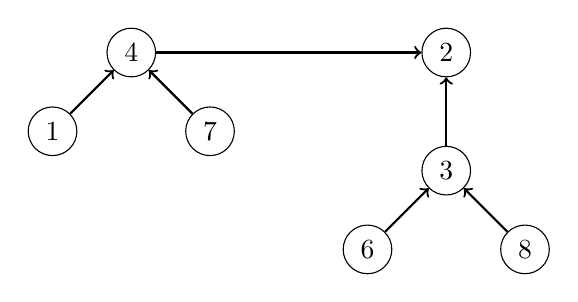
\begin{tikzpicture}
\node[draw, circle] (1) at (2,-1) {$1$};
\node[draw, circle] (2) at (7,0) {$2$};
\node[draw, circle] (3) at (7,-1.5) {$3$};
\node[draw, circle] (4) at (3,0) {$4$};
\node[draw, circle] (6) at (6,-2.5) {$6$};
\node[draw, circle] (7) at (4,-1) {$7$};
\node[draw, circle] (8) at (8,-2.5) {$8$};

\path[draw,thick,->] (1) -- (4);
\path[draw,thick,->] (7) -- (4);

\path[draw,thick,->] (3) -- (2);
\path[draw,thick,->] (6) -- (3);
\path[draw,thick,->] (8) -- (3);

\path[draw,thick,->] (4) -- (2);
\end{tikzpicture}
\end{center}

O conjunto resultante contém os elementos
$\{1,2,3,4,6,7,8\}$.
A partir daqui, o elemento 2 é o representante 
de todo o conjunto e o antigo representante 4 
aponta para o elemento 2.

A eficiência da estrutura union-find depende de 
como os conjuntos são unidos. 
Acontece que podemos seguir uma estratégia simples: 
sempre conectar o representante do conjunto 
\emph{menor} ao representante do conjunto \emph{maior} 
(ou, se os conjuntos forem do mesmo tamanho, 
podemos fazer uma escolha arbitrária). 
Usando esta estratégia, o comprimento de qualquer cadeia 
será $O(\log n)$, para que possamos 
encontrar o representante de qualquer elemento 
de forma eficiente, seguindo a cadeia correspondente.

\subsubsection{Implementação}

A estrutura union-find pode ser implementada 
usando arrays. 
Na implementação a seguir, 
o array \texttt{link} contém, para cada elemento, 
o próximo elemento 
na cadeia ou o próprio elemento se for 
um representante, 
e o array \texttt{size} indica para cada representante 
o tamanho do conjunto correspondente.

Inicialmente, cada elemento pertence a um conjunto separado:
\begin{lstlisting}
for (int i = 1; i <= n; i++) link[i] = i;
for (int i = 1; i <= n; i++) size[i] = 1;
\end{lstlisting}

A função \texttt{find} retorna 
o representante para um elemento $x$. 
O representante pode ser encontrado seguindo 
a cadeia que começa em $x$.

\begin{lstlisting}
int find(int x) {
    while (x != link[x]) x = link[x];
    return x;
}
\end{lstlisting}

A função \texttt{same} verifica 
se os elementos $a$ e $b$ pertencem ao mesmo conjunto. 
Isso pode ser feito facilmente usando a 
função \texttt{find}:

\begin{lstlisting}
bool same(int a, int b) {
    return find(a) == find(b);
}
\end{lstlisting}

\begin{samepage}
A função \texttt{unite} une os conjuntos 
que contêm os elementos $a$ e $b$ 
(os elementos devem estar em conjuntos diferentes). 
A função primeiro encontra os representantes 
dos conjuntos e então conecta o conjunto menor 
ao conjunto maior.

\begin{lstlisting}
void unite(int a, int b) {
    a = find(a);
    b = find(b);
    if (size[a] < size[b]) swap(a,b);
    size[a] += size[b];
    link[b] = a;
}
\end{lstlisting}
\end{samepage}

A complexidade de tempo da função \texttt{find} 
é $O(\log n)$, assumindo que o comprimento de cada 
cadeia é $O(\log n)$. 
Neste caso, as funções \texttt{same} e \texttt{unite} 
também funcionam em tempo $O(\log n)$. 
A função \texttt{unite} garante que o 
comprimento de cada cadeia seja $O(\log n)$ conectando 
o conjunto menor ao conjunto maior.

\section{Algoritmo de Prim}

\index{Algoritmo de Prim}

\index{Algoritmo de Prim}\footnote{O algoritmo foi 
nomeado em homenagem a R. C. Prim, que o publicou em 1957 \cite{pri57}.
No entanto, o mesmo algoritmo já havia sido descoberto em 1930
por V. Jarník.} é um método alternativo
para encontrar uma árvore geradora mínima.
O algoritmo primeiro adiciona um nó arbitrário
à árvore.
Depois disso, o algoritmo sempre escolhe
uma aresta de peso mínimo que
adiciona um novo nó à árvore.
Finalmente, todos os nós terão sido adicionados à árvore
e uma árvore geradora mínima terá sido encontrada.

O algoritmo de Prim se assemelha ao algoritmo de Dijkstra.
A diferença é que o algoritmo de Dijkstra sempre
seleciona uma aresta cuja distância do nó inicial
é mínima, mas o algoritmo de Prim simplesmente seleciona
a aresta de peso mínimo que adiciona um novo nó à árvore.

\subsubsection{Exemplo}

Vamos considerar como o algoritmo de Prim funciona
no seguinte grafo:

\begin{center}
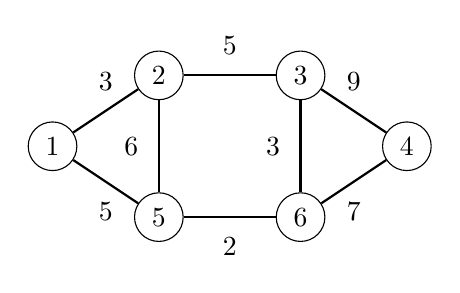
\begin{tikzpicture}[scale=0.9]
\node[draw, circle] (1) at (1.5,2) {$1$};
\node[draw, circle] (2) at (3,3) {$2$};
\node[draw, circle] (3) at (5,3) {$3$};
\node[draw, circle] (4) at (6.5,2) {$4$};
\node[draw, circle] (5) at (3,1) {$5$};
\node[draw, circle] (6) at (5,1) {$6$};
\path[draw,thick,-] (1) -- node[font=\small,label=above:3] {} (2);
\path[draw,thick,-] (2) -- node[font=\small,label=above:5] {} (3);
\path[draw,thick,-] (3) -- node[font=\small,label=above:9] {} (4);
\path[draw,thick,-] (1) -- node[font=\small,label=below:5] {} (5);
\path[draw,thick,-] (5) -- node[font=\small,label=below:2] {} (6);
\path[draw,thick,-] (6) -- node[font=\small,label=below:7] {} (4);
\path[draw,thick,-] (2) -- node[font=\small,label=left:6] {} (5);
\path[draw,thick,-] (3) -- node[font=\small,label=left:3] {} (6);

%\path[draw=red,thick,-,line width=2pt] (5) -- (6);
\end{tikzpicture}
\end{center}
Inicialmente, não há arestas entre os nós:
\begin{center}
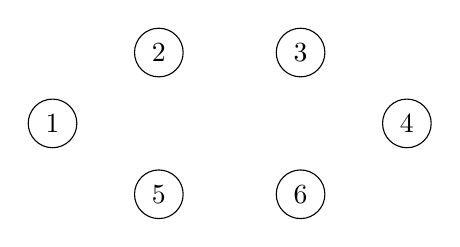
\begin{tikzpicture}[scale=0.9]
\node[draw, circle] (1) at (1.5,2) {$1$};
\node[draw, circle] (2) at (3,3) {$2$};
\node[draw, circle] (3) at (5,3) {$3$};
\node[draw, circle] (4) at (6.5,2) {$4$};
\node[draw, circle] (5) at (3,1) {$5$};
\node[draw, circle] (6) at (5,1) {$6$};
%\path[draw,thick,-] (1) -- node[font=\small,label=above:3] {} (2);
%\path[draw,thick,-] (2) -- node[font=\small,label=above:5] {} (3);
%\path[draw,thick,-] (3) -- node[font=\small,label=above:9] {} (4);
%\path[draw,thick,-] (1) -- node[font=\small,label=below:5] {} (5);
%\path[draw,thick,-] (5) -- node[font=\small,label=below:2] {} (6);
%\path[draw,thick,-] (6) -- node[font=\small,label=below:7] {} (4);
%\path[draw,thick,-] (2) -- node[font=\small,label=left:6] {} (5);
%\path[draw,thick,-] (3) -- node[font=\small,label=left:3] {} (6);
\end{tikzpicture}
\end{center}
Um nó arbitrário pode ser o nó inicial,
então vamos escolher o nó 1.
Primeiro, adicionamos o nó 2 que está conectado por
uma aresta de peso 3:
\begin{center}
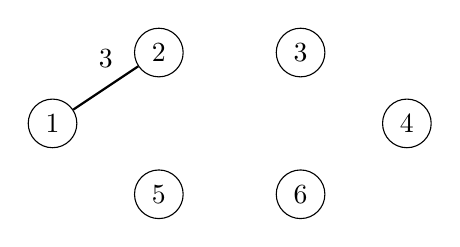
\begin{tikzpicture}[scale=0.9]
\node[draw, circle] (1) at (1.5,2) {$1$};
\node[draw, circle] (2) at (3,3) {$2$};
\node[draw, circle] (3) at (5,3) {$3$};
\node[draw, circle] (4) at (6.5,2) {$4$};
\node[draw, circle] (5) at (3,1) {$5$};
\node[draw, circle] (6) at (5,1) {$6$};
\path[draw,thick,-] (1) -- node[font=\small,label=above:3] {} (2);
%\path[draw,thick,-] (2) -- node[font=\small,label=above:5] {} (3);
%\path[draw,thick,-] (3) -- node[font=\small,label=above:9] {} (4);
%\path[draw,thick,-] (1) -- node[font=\small,label=below:5] {} (5);
%\path[draw,thick,-] (5) -- node[font=\small,label=below:2] {} (6);
%\path[draw,thick,-] (6) -- node[font=\small,label=below:7] {} (4);
%\path[draw,thick,-] (2) -- node[font=\small,label=left:6] {} (5);
%\path[draw,thick,-] (3) -- node[font=\small,label=left:3] {} (6);
\end{tikzpicture}
\end{center}

Depois disso, existem duas arestas com peso 5,
então podemos adicionar o nó 3 ou o nó 5 à árvore.
Vamos adicionar o nó 3 primeiro:
\begin{center}
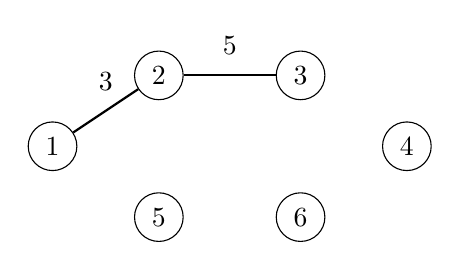
\begin{tikzpicture}[scale=0.9]
\node[draw, circle] (1) at (1.5,2) {$1$};
\node[draw, circle] (2) at (3,3) {$2$};
\node[draw, circle] (3) at (5,3) {$3$};
\node[draw, circle] (4) at (6.5,2) {$4$};
\node[draw, circle] (5) at (3,1) {$5$};
\node[draw, circle] (6) at (5,1) {$6$};
\path[draw,thick,-] (1) -- node[font=\small,label=above:3] {} (2);
\path[draw,thick,-] (2) -- node[font=\small,label=above:5] {} (3);
%\path[draw,thick,-] (3) -- node[font=\small,label=above:9] {} (4);
%\path[draw,thick,-] (1) -- node[font=\small,label=below:5] {} (5);
%\path[draw,thick,-] (5) -- node[font=\small,label=below:2] {} (6);
%\path[draw,thick,-] (6) -- node[font=\small,label=below:7] {} (4);
%\path[draw,thick,-] (2) -- node[font=\small,label=left:6] {} (5);
%\path[draw,thick,-] (3) -- node[font=\small,label=left:3] {} (6);
\end{tikzpicture}
\end{center}

\begin{samepage}
O processo continua até que todos os nós tenham sido incluídos na árvore:
\begin{center}
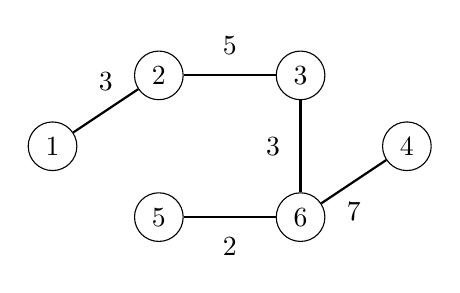
\begin{tikzpicture}[scale=0.9]
\node[draw, circle] (1) at (1.5,2) {$1$};
\node[draw, circle] (2) at (3,3) {$2$};
\node[draw, circle] (3) at (5,3) {$3$};
\node[draw, circle] (4) at (6.5,2) {$4$};
\node[draw, circle] (5) at (3,1) {$5$};
\node[draw, circle] (6) at (5,1) {$6$};
\path[draw,thick,-] (1) -- node[font=\small,label=above:3] {} (2);
\path[draw,thick,-] (2) -- node[font=\small,label=above:5] {} (3);
%\path[draw,thick,-] (3) -- node[font=\small,label=above:9] {} (4);
%\path[draw,thick,-] (1) -- node[font=\small,label=below:5] {} (5);
\path[draw,thick,-] (5) -- node[font=\small,label=below:2] {} (6);
\path[draw,thick,-] (6) -- node[font=\small,label=below:7] {} (4);
%\path[draw,thick,-] (2) -- node[font=\small,label=left:6] {} (5);
\path[draw,thick,-] (3) -- node[font=\small,label=left:3] {} (6);
\end{tikzpicture}
\end{center}
\end{samepage}

\subsubsection{Implementação}

Assim como o algoritmo de Dijkstra, o algoritmo de Prim pode ser
implementado eficientemente usando uma fila de prioridade.
A fila de prioridade deve conter todos os nós
que podem ser conectados ao componente atual usando
uma única aresta, em ordem crescente dos pesos
das arestas correspondentes.

A complexidade de tempo do algoritmo de Prim é
$O(n + m \log m)$ que é igual à complexidade de tempo
do algoritmo de Dijkstra.
Na prática, os algoritmos de Prim e Kruskal
são ambos eficientes, e a escolha do algoritmo
é uma questão de gosto.
Ainda assim, a maioria dos programadores competitivos usam o algoritmo de Kruskal.